\subsubsection{21.11.2015}
\textit{\textbf{Time frame:}} 17:00-21:30 \newline
The mechanism for shifting the bucket was finished. 
The gripper was recreated due to the increasing of the height of the robot after installing 10 cm wheels. The axis was moved to the demanded height. After that there was created the brush. It was made of silicone tubes tied to the axis by plastic clamps. Next, the gripper was tested. The brush was capable of collecting debris. As for continious rotation servo, it was too slow and didn't have enough torque for acceptable collecing of the debris. One more problem was that the gripper was staggering, because it was made of two axes connected by the sleeve. To avoid this, it was decided to install one tetrix tube instead of axes.

\begin{figure}[H]
	\begin{minipage}[h]{0.47\linewidth}
		\center{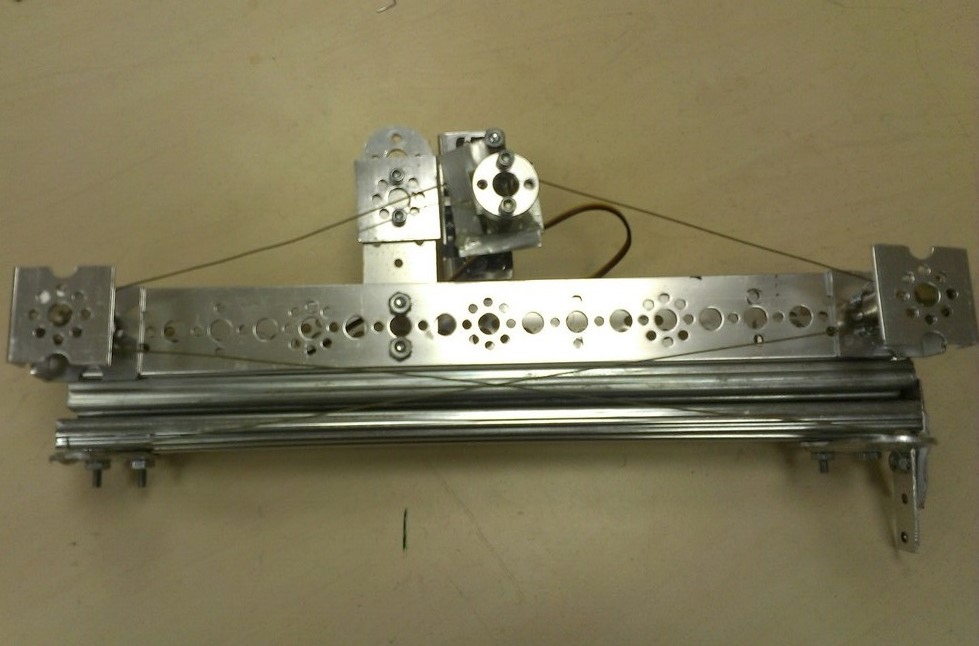
\includegraphics[scale=0.2]{3Engineering/5Team_meetings/days_of_meetings/2015.11.21/images/01}}
		\caption{Mechanism for shifting the bucket}
	\end{minipage}
	\hfill
	\begin{minipage}[h]{0.47\linewidth}
		\center{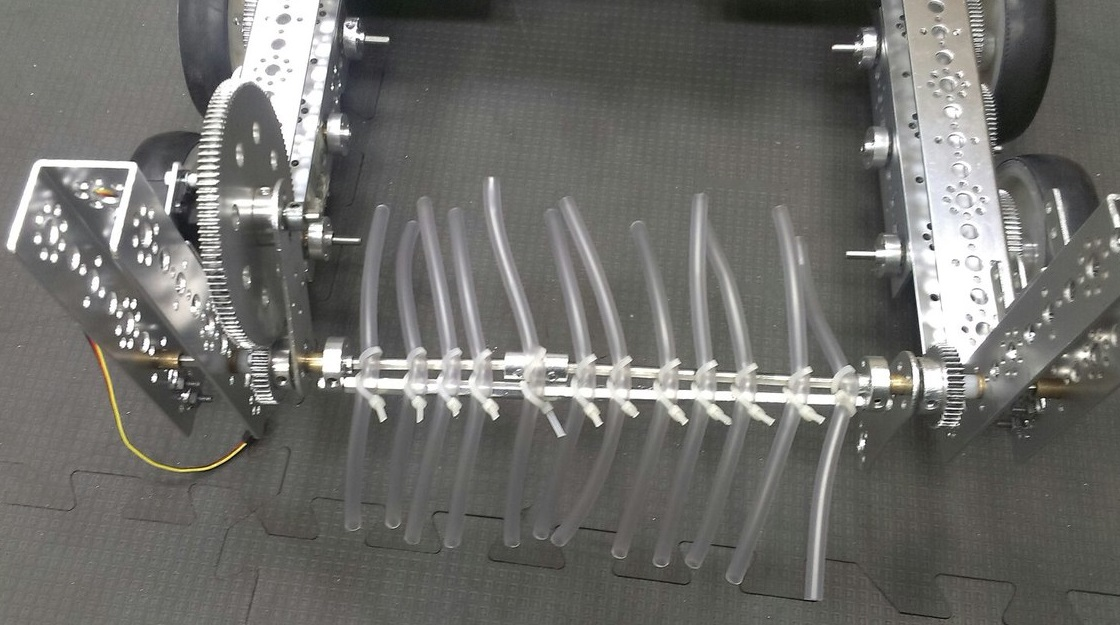
\includegraphics[scale=0.2]{3Engineering/5Team_meetings/days_of_meetings/2015.11.21/images/02}}
		\caption{Gripper with the brush}
	\end{minipage}
\end{figure}
